\tikzset{every picture/.style={line width=0.75pt}} %set default line width to 0.75pt

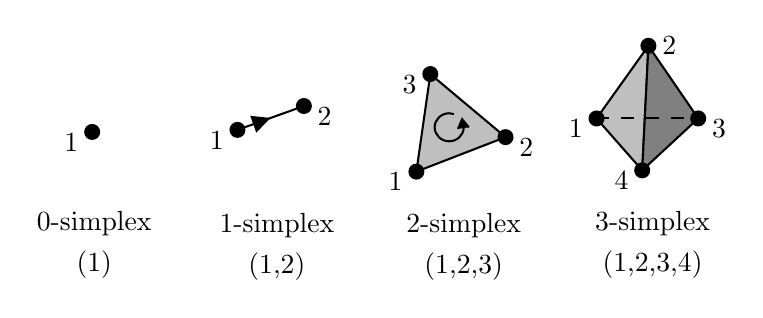
\begin{tikzpicture}[x=0.75pt,y=0.75pt,yscale=-1,xscale=1]

\coordinate (01) at (77,72);
\coordinate (11) at (147,71);
\coordinate (12) at (179,59.5);
\coordinate (21) at (233.21,91.12);
\coordinate (22) at (276.15,74.49);
\coordinate (23) at (239.92,44.11);
\coordinate (31) at (320,65.5);
\coordinate (32) at (345,30.5);
\coordinate (33) at (369,65.5);
\coordinate (34) at (342,90.5);

% 0 Simplex
\draw   [black, fill=black] (01) circle [radius= 3.35] ;

% 1 Simplex
\draw   [black, fill=black] (11) circle [radius= 3.35] ;
\draw   [black, fill=black] (12) circle [radius= 3.35] ;
\draw   (11) -- (12) ;

% 2 Simplex
\draw   [black, fill=lightgray] (21) -- (22) -- (23) -- cycle   ;
\draw   [black, fill=black] (21) circle [radius= 3.35] ;
\draw   [black, fill=black] (22) circle [radius= 3.35] ;
\draw   [black, fill=black] (23) circle [radius= 3.35] ;

% 3 Simplex
\draw   [black, fill=lightgray] (31) -- (32) -- (34) -- cycle   ;
\draw   [black, fill=gray]      (32) -- (33) -- (34) -- cycle   ;
\draw   [dash pattern={on 4.5pt off 4.5pt}]  (31) -- (33) ;
\draw   [black, fill=black] (31) circle [radius= 3.35] ;
\draw   [black, fill=black] (32) circle [radius= 3.35] ;
\draw   [black, fill=black] (33) circle [radius= 3.35] ;
\draw   [black, fill=black] (34) circle [radius= 3.35] ;

% Straight Arrow
\draw [shift={(163,65.25)}, rotate = 520.23] [fill={rgb, 255:red, 0; green, 0; blue, 0 }  ][line width=0.08]  [draw opacity=0] (8.93,-4.29) -- (0,0) -- (8.93,4.29) -- cycle    ;

% Circle Arrow
\draw  [draw opacity=0] (255.97,69.08) .. controls (255.99,69.3) and (256,69.52) .. (256,69.75) .. controls (256,73.48) and (252.87,76.5) .. (249,76.5) .. controls (245.13,76.5) and (242,73.48) .. (242,69.75) .. controls (242,66.02) and (245.13,63) .. (249,63) .. controls (249.81,63) and (250.59,63.13) .. (251.32,63.38) -- (249,69.75) -- cycle ; \draw   (255.97,69.08) .. controls (255.99,69.3) and (256,69.52) .. (256,69.75) .. controls (256,73.48) and (252.87,76.5) .. (249,76.5) .. controls (245.13,76.5) and (242,73.48) .. (242,69.75) .. controls (242,66.02) and (245.13,63) .. (249,63) .. controls (249.81,63) and (250.59,63.13) .. (251.32,63.38) ;
\draw  [fill={rgb, 255:red, 0; green, 0; blue, 0 }  ,fill opacity=1 ] (253.25,70.52) -- (255.25,65.85) -- (258.47,69.77) ;


% Caption Labels
\draw (78,116)   node   [align=left] {0-simplex};
\draw (166,117)  node   [align=left] {1-simplex};
\draw (256,117)  node   [align=left] {2-simplex};
\draw (347,116)  node   [align=left] {3-simplex};
\draw (78,136)   node   [align=left] {(1)};
\draw (166,137)  node   [align=left] {(1,2)};
\draw (256,137)  node   [align=left] {(1,2,3)};
\draw (347,136)  node   [align=left] {(1,2,3,4)};

% Vertex Labels
\draw (01)+(-10,5)  node   [align=left] {1};
\draw (11)+(-10,5)  node   [align=left] {1};
\draw (12)+(10,5)   node   [align=left] {2};
\draw (21)+(-10,5)  node   [align=left] {1};
\draw (22)+(10,5)   node   [align=left] {2};
\draw (23)+(-10,5)  node   [align=left] {3};
\draw (31)+(-10,5)  node   [align=left] {1};
\draw (32)+(10,0)   node   [align=left] {2};
\draw (33)+(10,5)   node   [align=left] {3};
\draw (34)+(-10,5)  node   [align=left] {4};




\end{tikzpicture}
